%=============================================================
%  main.tex  ―  修士論文メインファイル
%  Engine : LuaLaTeX
%  Class  : jlreq (日本語組版規則準拠)
%  Bib    : BibLaTeX + biber
%
%  コンパイル手順:
%    lualatex main && biber main && lualatex main && lualatex main
%=============================================================

\documentclass[
  book,                   % book モード（\chapter, \mainmatter が使える）
  paper        = a4,
  fontsize     = 12pt,
  head_space   = 30mm,
  gutter       = 30mm,    % 綴じ側余白
  line_length  = 40zw,    % 1行の文字数
  number_of_lines = 36,   % 1ページの行数
  titlepage,
  twoside,
]{jlreq}

% ── プリアンブル（パッケージ・設定）──────────────────────────
%=============================================================
%  preamble.tex  ―  パッケージ・設定・マクロ定義
%=============================================================

% ── 日本語フォント（LuaLaTeX） ───────────────────────────────
% luatexja-preset が luatexja-fontspec を内包するので単独でロード
% macOS (Hiragino フォント): hiragino-pron
% Linux/CI (Noto フォント) : noto
\usepackage[hiragino-pron]{luatexja-preset}

% ── 数式 ──────────────────────────────────────────────────────
\usepackage{amsmath}
\usepackage{amssymb}
\usepackage{mathtools}

% ── 図・表 ────────────────────────────────────────────────────
\usepackage{graphicx}
\graphicspath{{figures/}}           % 図の検索パス
\usepackage{booktabs}               % \toprule, \midrule, \bottomrule
\usepackage{threeparttable}         % 表の注釈
\usepackage{longtable}              % 複数ページにまたがる表
\usepackage{multirow}               % セル結合
\usepackage{array}                  % 列幅指定 (>{...}p{...} など)
\usepackage{tabularx}               % 幅指定表
\usepackage{float}                  % [H] 指定
\usepackage{caption}
\captionsetup{
  font       = small,
  labelfont  = bf,
  format     = hang,
  width      = 0.9\linewidth,
}
\captionsetup[table]{position=above}
\captionsetup[figure]{position=below}

% ── 数値・単位 ────────────────────────────────────────────────
\usepackage{siunitx}
\sisetup{
  group-separator   = {,},
  group-minimum-digits = 4,
}

% ── ハイパーリンク ───────────────────────────────────────────
\usepackage[
  colorlinks = true,
  linkcolor  = black,
  citecolor  = black,
  urlcolor   = black,
  bookmarks  = true,
]{hyperref}
\usepackage{url}

% ── 文献 (BibLaTeX) ──────────────────────────────────────────
\usepackage[
  style       = apa,      % APA形式（経済学・経営学の標準）
  backend     = biber,
  natbib      = true,     % \citep, \citet が使える
  sortcites   = true,
  maxcitenames = 2,
  maxbibnames  = 99,
]{biblatex}

% ── カラー・強調 ─────────────────────────────────────────────
\usepackage{xcolor}
\definecolor{myblue}{RGB}{46, 64, 87}
\definecolor{myred}{RGB}{180, 50, 50}

% ── コード表示 ────────────────────────────────────────────────
\usepackage{listings}
\lstset{
  basicstyle   = \ttfamily\small,
  keywordstyle = \color{myblue}\bfseries,
  commentstyle = \color{gray}\itshape,
  stringstyle  = \color{myred},
  numbers      = left,
  numberstyle  = \tiny\color{gray},
  frame        = single,
  breaklines   = true,
  captionpos   = b,
}

% ── その他 ────────────────────────────────────────────────────
\usepackage{setspace}
\setstretch{1.5}           % 行間を 1.5 倍（修論標準: 1.5〜1.6）
\usepackage{enumitem}
\usepackage{pdfpages}      % 外部PDFの取り込み（付録用）

% ── ヘッダ・フッタ ───────────────────────────────────────────
% \usepackage{jlreq-deluxe}  % jlreq用の見出しスタイル拡張（インストール済みなら有効化）
% ヘッダ・フッタのカスタマイズは jlreq の \ModifyHeading 等で行う

%=============================================================
% カスタムマクロ
%=============================================================

% 統計用記号
\newcommand{\AUC}{\mathrm{AUC}}
\newcommand{\SHAP}{\mathrm{SHAP}}
\newcommand{\XGB}{\textrm{XGBoost}}
\newcommand{\Cluster}[1]{\textbf{C#1}}   % \Cluster{0} → C0

% 注釈記号（表内）
\newcommand{\sig}[1]{$^{#1}$}  % \sig{***}

% TODO マーカー（執筆中のみ表示）
\newcommand{\TODO}[1]{\textcolor{red}{\textbf{[TODO: #1]}}}

% 引用ショートカット
% \tcite{key} → 著者 (年) のインライン引用
\newcommand{\tcite}[1]{\citeauthor{#1} (\citeyear{#1})}


% ── 文献データベース ──────────────────────────────────────────
\addbibresource{references.bib}

%=============================================================
\begin{document}
%=============================================================

% ── 表紙 ────────────────────────────────────────────────────
\begin{titlepage}
  \centering
  \vspace*{40mm}
  {\Large 九州大学大学院 経済学府\par}
  \vspace{8mm}
  {\large 経済システム専攻\par}
  \vspace{20mm}
  {\LARGE\bfseries 日本上場企業の財務クラスター遷移分析\par}
  \vspace{6mm}
  {\large ――機械学習を用いた遷移要因の解明――\par}
  \vspace{30mm}
  {\large 修士論文\par}
  \vspace{20mm}
  {\large 提出年月：2026年〇月\par}
  \vspace{10mm}
  {\large 氏名：〇〇〇〇\par}
  \vspace{6mm}
  {\large 指導教員：〇〇〇〇 教授\par}
  \vfill
\end{titlepage}

% ── 概要（和文アブストラクト）───────────────────────────────
\cleardoublepage
\chapter*{概要}
\addcontentsline{toc}{chapter}{概要}
% TODO: 概要を記述する（400〜600字程度）
\bigskip
本稿では，日本上場企業の財務データを用いてクラスタリングと遷移分析を行い，
企業の財務構造がどのように変化するかを機械学習によって解明する。
%
% （ここに概要を執筆）

% ── 目次 ────────────────────────────────────────────────────
\cleardoublepage
\tableofcontents

% ── 図目次・表目次 ───────────────────────────────────────────
\cleardoublepage
\listoffigures
\listoftables

%=============================================================
% 本文
%=============================================================
\mainmatter   % jlreq: ページ番号をアラビア数字に切り替え

%=============================================================
%  第1章 はじめに
%=============================================================
\chapter{はじめに}
\label{chap:intro}

\section{研究背景}
\label{sec:intro-background}

企業の財務構造は静的なものではない。
企業は誕生から成長，成熟，そして衰退に至るライフサイクルの各段階において，
資産構成，負債構造，収益パターン，キャッシュフローの構造を体系的に変化させる。
\tcite{Mueller1972} は産業組織論の観点から企業ライフサイクル理論を提唱し，
経営者の投資行動と利益分配がライフサイクル段階に依存することを理論的に示した。
その後，\tcite{Dickinson2011} は営業・投資・財務キャッシュフローの
符号パターンに基づく5段階分類（導入期・成長期・成熟期・動揺期・衰退期）を提案し，
企業ライフサイクルの実証的な測定手法として広く採用されるに至った。
\tcite{Habib2019survey} のサーベイが示すように，この枠組みは現在，
会計・財務・コーポレートガバナンスの各分野における研究の基盤として機能している。

ライフサイクル理論によれば，企業の財務政策は段階に応じて体系的に変化する。
\tcite{DeAngelo2006} は配当政策がライフサイクル段階に依存することを，
\tcite{Hirsch2011} は負債水準が段階に応じて変化することを示した。
\tcite{Faff2016} は配当・投資・資金調達・現金保有の4つの財務政策が
ライフサイクルに沿って共変動することを包括的に実証している。
こうした知見は，企業の財務構造が単一の指標ではなく
多変量的な特性として捉えるべきであること，
そしてその特性がライフサイクルに沿って動態的に変化することを示唆する。

日本経済は本研究の分析期間（2010〜2024年度）において，
複数の構造的変化を経験した。
1990年代のバブル崩壊後に始まった長期停滞（いわゆる「失われた30年」）の中で，
日本企業は内部留保の蓄積と負債の圧縮を進め，
財務構造は全体として保守化の傾向を示してきた。
2012年末に始まったアベノミクスと日本銀行による異次元金融緩和（量的・質的金融緩和）は，
企業の資金調達環境を大きく変容させた。
超低金利環境の長期化は企業の借入コストを歴史的低水準に押し下げ，
負債構造に影響を与えたと考えられる。
一方で，コーポレートガバナンス・コードの導入（2015年）は，
上場企業に対してROE目標の設定や政策保有株式の縮減を促し，
資本効率性に対する市場の要請を強めた。

さらに，2020年以降の COVID-19 パンデミックは，
業種によって非対称的な影響をもたらした。
飲食・宿泊・運輸業など対面サービス業は急激な収益悪化に直面する一方，
情報通信業やEC関連企業はデジタルトランスフォーメーション（DX）の
加速により成長機会を獲得した。
こうしたマクロ経済環境の変動と制度変更は，企業の財務構造の変化パターン
――すなわち，どのような企業がどのような財務状態に遷移するか――に
影響を与えている可能性がある。
本研究が対象とする15年間は，このように多様な構造変化を含む期間であり，
企業の財務構造ダイナミクスを分析するうえで豊富な変動情報を提供する。

しかし，既存の企業ライフサイクル研究および財務分類研究の多くは，
ある時点における企業の分類に焦点を当てており，
企業が年度をまたいでどのように財務構造を変化させるか
――すなわち，クラスター間の遷移――については十分に解明されていない。
\tcite{GonzalezRuiz2021} は K-Means クラスタリングとマルコフ連鎖を用いた遷移分析を
試みた先駆的研究であるが，対象は 35 社に限定されており，
遷移を引き起こす要因の体系的な解明には至っていない。
また，既存研究の多くは米国や欧州の企業を対象としており，
日本上場企業の財務構造遷移に関する大規模な実証分析は行われていない。

日本の上場企業は，有価証券報告書を通じて継続的かつ標準化された形式で
財務データが開示されている。
金融商品取引法に基づくこの開示制度は，
企業横断的・時系列的に整合性のある財務データを提供しており，
パネルデータ分析の基盤として優れた環境を形成している。
約 \num{3558} 社・15 年間の大規模パネルデータを活用することで，
米国や欧州を対象とした既存研究を補完し，
日本企業に固有の財務構造ダイナミクスを解明する実証分析が可能となる。

近年，機械学習手法の財務分析への応用が急速に進展している。
特に，勾配ブースティング手法である XGBoost \citep{ChenGuestrin2016} は，
倒産予測をはじめとする財務予測タスクにおいて伝統的な統計モデルを上回る
予測精度を達成することが実証されている \citep{Nguyen2023, BenJabeur2023}。
また，SHAP（Shapley Additive Explanations; \citealt{LundbergLee2017}）との
組み合わせにより，高い予測精度を維持しつつモデルの解釈可能性を確保する
フレームワークが確立されつつある \citep{Zhang2023}。
SHAP は協力ゲーム理論における Shapley 値 \citep{Shapley1953} に基礎を置き，
各特徴量の予測への貢献度を理論的に正当化された方法で定量化する。
これらの手法を財務クラスター遷移の分析に応用することで，
どの財務変数が遷移と関連し，遷移先の予測に寄与するかを定量的に解明できる可能性がある。

\section{研究課題}
\label{sec:intro-questions}

以上の背景を踏まえ，本研究では以下の3つの研究課題（RQ）を設定する。

\begin{description}[style=nextline, leftmargin=2em]
  \item[\textbf{RQ1}] 日本上場企業の財務構造は，年度をまたいでどのようなクラスターを形成し，
    各クラスターはどの程度安定的に維持されるか。
\end{description}

企業のライフサイクルに関する理論的予測によれば，
財務構造は段階的に変化するため，ある程度の安定性を示すことが期待される。
しかし，\tcite{Dickinson2011} のキャッシュフロー分類とは異なり，
11の財務変数に基づくデータ駆動型の分類において
どの程度の安定性が観察されるかは実証的な問いである。
クラスターの安定性の程度は，財務構造が戦略的・構造的に決定されているのか，
それとも短期的なショックに応じて頻繁に変化するのかを識別する手がかりとなる。

\begin{description}[style=nextline, leftmargin=2em]
  \item[\textbf{RQ2}] クラスター間の遷移（財務構造の変化）は，
    どの財務変数と関連しているか。
\end{description}

企業がある財務クラスターから別のクラスターへ移行する際に，
どの財務指標の変化がその遷移と関連しているかを明らかにすることは，
ライフサイクル理論の実証的な検証に寄与する。
\tcite{DeAngelo2006} は配当政策が，\tcite{Hirsch2011} は負債水準が，
それぞれライフサイクル段階と関連することを示しているが，
複数の財務変数を同時に考慮した場合にどの変数が相対的に重要であるかは未解明である。

\begin{description}[style=nextline, leftmargin=2em]
  \item[\textbf{RQ3}] 遷移が生じた場合，遷移先クラスターはどの財務変数によって
    予測されるか。また，遷移先によって関連する要因は異なるか。
\end{description}

遷移の有無だけでなく，遷移先を予測できるかどうかは，
経営戦略や財務政策の観点から重要な問いである。
財務脆弱クラスターへの遷移と大企業クラスターへの遷移では，
関連する財務変数が異なる可能性がある。
こうした非対称性の存在は，企業の財務構造変化が単一のメカニズムでは
説明できないことを示唆し，遷移先に応じた差別化された理解の必要性を提起する。

RQ1 は PCA + K-Means クラスタリングとハンガリアン法によるラベル整合
（第\ref{chap:data-method}章）を通じて検討する。
RQ2 は二値プロビット分析および XGBoost の二値分類モデル + SHAP 分析により，
RQ3 は多項ロジット分析および XGBoost の多クラス分類モデル + SHAP 分析により，
それぞれ検討する。

\section{本研究の貢献}
\label{sec:intro-contribution}

本研究は，以下の3点で既存研究に対して貢献する。

\begin{enumerate}
  \item \textbf{方法論的貢献――既存手法の創意的な組み合わせによる
    時系列的追跡可能性の実現}：
    PCA による次元削減，K-Means クラスタリング \citep{Lloyd1982}，
    およびハンガリアン法 \citep{Kuhn1955} による年度間ラベル整合を組み合わせることで，
    年度をまたいで追跡可能な財務クラスターを定義する手法を構築した。
    各手法は確立された技術であるが，これらを統合して年度間の
    クラスター対応関係を客観的に確立する枠組みは，
    財務クラスター遷移分析の文脈では新規の試みである。

  \item \textbf{実証的貢献――日本上場企業の財務クラスター構造と
    遷移パターンの記述}：
    日本上場企業 \num{3558} 社・15 年間のパネルデータを用いて，
    財務クラスター遷移の実態を体系的に記述した。
    分析の結果，5つの財務クラスターが識別され，
    年度間の自己遷移率が高い水準にあることが明らかになった。
    この強いパス依存性は，企業の財務構造が短期的なショックよりも
    構造的な要因によって規定されていることを示唆する。
    なお，二値プロビット分析における説明力（Pseudo $R^2$ = 0.043）は低く，
    個々の財務変数の水準のみからでは遷移の有無を十分に説明できないことも示された。
    この結果は，遷移の発生が財務変数の水準よりも変化の方向やタイミングに
    依存している可能性を示唆する。

  \item \textbf{予測的貢献――XGBoost + SHAP による遷移要因の定量的解明}：
    XGBoost と SHAP を用いた2段階予測モデルにより，
    遷移の有無と遷移先の双方について，関連する財務変数を特定した。
    SHAP 分析により，遷移先クラスターごとに異なる財務変数が予測に寄与すること
    ――遷移の非対称性――が明らかになった。
    この非対称性は，企業の財務構造変化が多元的なメカニズムに
    駆動されていることを示唆する。
    ただし，SHAP 値は予測への貢献度を示すものであり，
    因果関係を意味するものではない点に留意が必要である。
\end{enumerate}

\section{論文の構成}
\label{sec:intro-structure}

本論文の構成は以下のとおりである。

第\ref{chap:literature}章では，企業ライフサイクル理論，財務政策とライフサイクルの関係，
財務クラスタリングと機械学習に関する先行研究を概観し，
本研究の位置づけと既存研究に対するギャップを明らかにする。

第\ref{chap:data-method}章では，分析に用いるデータ（日本上場企業 \num{3558} 社，
2010〜2024年度）の概要と前処理手順，および PCA + K-Means クラスタリング，
ハンガリアン法によるラベル整合，二値プロビット，多項ロジット，
XGBoost + SHAP の各分析手法を詳述する。

第\ref{chap:results}章では，5クラスターの特性，遷移行列，
二値・多クラス予測モデルの性能，SHAP による特徴量重要度，
およびロバストネスチェックの結果を報告する。

第\ref{chap:discussion}章では，各クラスターの経済的解釈，
パス依存性のメカニズム，遷移の非対称性について先行研究と対比しつつ考察し，
投資家・経営者・政策立案者への含意を論じる。

第\ref{chap:conclusion}章では，研究成果を要約し，学術的貢献を整理した上で，
本研究の限界と今後の研究方向を述べる。

%=============================================================
%  第2章 先行研究
%=============================================================
\chapter{先行研究}
\label{chap:literature}

\section{企業ライフサイクル論}
\label{sec:lit-lifecycle}

\subsection{ライフサイクルの概念と測定}

企業ライフサイクル理論の源流は，\tcite{Mueller1972} の産業組織論的アプローチに遡る。
Mueller は，企業が誕生・成長・成熟・衰退という段階を経る過程で，
経営者の投資行動や利益分配が体系的に変化することを理論的に示した。
この枠組みは，企業の財務政策がライフサイクル段階に依存するという考え方の基礎を形成している。

\tcite{Anthony1992} は，会計情報の有用性がライフサイクル段階によって異なることを実証した。
同研究は売上高成長率・設備投資比率・配当支払率を代理変数として企業を成長期・成熟期・衰退期に
分類し，各段階で株価と利益・売上高の関連性が異なることを示した。
この知見は，企業の財務特性がライフサイクルに沿って構造的に変化することを支持する。

\tcite{Dickinson2011} は，営業・投資・財務キャッシュフローの符号パターンに基づいて
企業を5段階のライフサイクル（導入期・成長期・成熟期・動揺期・衰退期）に分類する
手法を提案した。同研究は，この分類が企業の収益性・成長性・配当政策と整合することを示し，
企業ライフサイクル代理変数として広く採用されるに至った。
本研究における5クラスター分類は，Dickinson の5段階分類と概念的に対応するが，
キャッシュフローの符号パターンではなく，11の財務変数に基づくデータ駆動型の分類である点で異なる。

\tcite{Habib2019survey} はライフサイクル研究を包括的にサーベイし，
会計・財務・コーポレートガバナンスの各分野でライフサイクル概念がどのように
応用されてきたかを整理した。
同サーベイは，ライフサイクル研究が配当政策，資本構造，リスクテイキング，M\&A，
資本コストなど多岐にわたる企業行動の説明に有効であることを確認している。

\subsection{財務政策とライフサイクル}

\paragraph{配当政策}
\tcite{DeAngelo2006} は，企業のライフサイクル段階が配当政策を規定するという
ライフサイクル仮説を実証的に検証した。同研究は，利益剰余金と払込資本の比率
（RE/TE ratio）が配当支払いの傾向を強く予測することを示し，
成熟企業ほど配当を支払う傾向があることを明らかにした。
\tcite{Fama2001} は米国上場企業において配当支払企業の割合が長期的に減少している現象を
記述し，その主因が企業特性の変化（小規模・低収益・高成長企業の増加）にあることを示した。
\tcite{Denis2008} は国際的なデータを用いて，配当支払いの決定要因がライフサイクル段階と
整合することを確認した。
これらの知見は，本研究のクラスター間で観察される配当関連指標の差異が，
ライフサイクル段階の差異を反映している可能性を示唆する。

\paragraph{資本構造}
ライフサイクルに沿った資本構造の変化も広く研究されている。
\tcite{Hirsch2011} は，企業のライフサイクル段階に応じて最適な負債水準が異なることを
理論的に示した。成長期の企業は内部資金と株式発行を優先し，
成熟期の企業はフリーキャッシュフローの規律づけとして負債を活用する傾向がある。
\tcite{Castro2016} は欧州上場企業のパネルデータを用いて，
目標レバレッジとその調整速度がライフサイクル段階によって異なることを実証した。
本研究において，\Cluster{2}（財務優良型）と \Cluster{0}（標準型）の自己資本比率の差異は，
こうしたライフサイクルに沿った資本構造の違いを反映していると考えられる。

\paragraph{リスクテイキング}
\tcite{Habib2017} は，企業のリスクテイキング行動がライフサイクル段階と投資家心理の
双方に依存することを示した。導入期・衰退期の企業はリスクテイキング水準が高く，
成熟期の企業はそれが低い傾向にある。
\tcite{Faff2016} は配当・投資・資金調達・現金保有の4つの財務政策が
ライフサイクルに沿って体系的に変化することを包括的に実証した。
これらの知見は，本研究のクラスター遷移が企業のリスク・プロファイルの変化と
関連している可能性を支持する。

\section{財務クラスタリングと機械学習}
\label{sec:lit-clustering}

\subsection{財務指標によるクラスタリング}

財務指標に基づく企業の分類は長い研究の歴史を持つ。
\tcite{Gupta1972} は財務比率のクラスター分析により産業特性を捉えることを試み，
\tcite{Pinches1973} は財務パターンの時系列的安定性を検証した。
これらの初期研究は，財務指標に基づく企業分類が経済的に意味のあるグループを
形成しうることを示している。

\tcite{GonzalezRuiz2021} は K-Means クラスタリングとマルコフ連鎖を組み合わせ，
企業の信用品質クラスター間の遷移確率を推定した。
本研究の方法論と最も類似しており，クラスタリング＋遷移分析の先駆的研究として位置づけられる。
ただし同研究は35社と小規模な分析に留まっており，日本の上場企業全体を対象とした
大規模分析は行われていない。

\tcite{Li2022} は PCA と K-Means の組み合わせにより企業財務リスクの識別を行い，
高リスク企業と低リスク企業のクラスターを識別することに成功した。

\tcite{Fodor2021} は株式リターンの相関構造に基づく財務クラスターが
産業分類とは異なるグループ構造を捉えることを示した。
この知見は，財務データに基づくクラスタリングが従来の産業分類では捉えきれない
企業間の類似性を明らかにしうることを示唆しており，
本研究が産業分類ではなくデータ駆動型のクラスタリングを採用する根拠の一つとなる。

\subsection{機械学習を用いた財務予測}

倒産予測の分野では，機械学習手法の優位性が実証されている。
\tcite{Shumway2001} はハザードモデルの枠組みを提案して以来，
動的モデルが静的モデルを上回ることが示されてきた。
近年では，勾配ブースティング手法が特に高い予測精度を達成している。

\tcite{Nguyen2023} は Random Forest, LightGBM, XGBoost, NGBoost を
比較し，XGBoost が AUC 約 94\% を達成することを示した。
同研究はさらに SHAP（Shapley Additive Explanations）を用いて
各変数の貢献度を定量化し，モデルの解釈可能性を確保した。

\tcite{BenJabeur2023} は特徴量重要度に基づく変数選択（FS-XGBoost）を提案し，
財務比率の選択がモデル精度に与える影響を分析した。
適切な特徴量選択がモデルの汎化性能を向上させることを示している。

\tcite{Zhang2023} は XGBoost に証拠理論を組み合わせた財務リスク早期警戒モデルを構築し，
SHAP により各変数の方向性を定量化した。

これらの研究は，XGBoost + SHAP の組み合わせが財務予測において
高精度かつ解釈可能なフレームワークを提供することを示している。
しかし，既存研究は倒産予測やリスク分類を対象としており，
財務クラスター間の遷移を予測する枠組みは提示されていない。

\section{本研究の位置づけ}
\label{sec:lit-position}

既存研究との対比を表\ref{tab:lit-comparison}に示す。

\begin{table}[htbp]
  \centering
  \caption{先行研究との比較}
  \label{tab:lit-comparison}
  \small
  \begin{tabularx}{\linewidth}{lXXcc}
    \toprule
    研究 & 手法 & データ & 遷移分析 & 要因解明 \\
    \midrule
    \tcite{Dickinson2011} & CF パターン & 米国上場 & なし & なし \\
    \tcite{GonzalezRuiz2021} & K-Means + Markov & 35社 & あり & なし \\
    \tcite{Li2022} & PCA + K-Means & 中国上場 & なし & なし \\
    \tcite{Nguyen2023} & XGBoost + SHAP & フランス企業 & なし & あり \\
    \textbf{本研究} & PCA + K-Means + XGBoost + SHAP & 日本上場 3,558社 & \textbf{あり} & \textbf{あり} \\
    \bottomrule
  \end{tabularx}
\end{table}

本研究は，以下の3点において既存研究を拡張する。
第一に，\num{3558} 社・15 年間の大規模な日本企業パネルデータを用いることで，
\tcite{GonzalezRuiz2021} の小規模分析（35社）を規模面で大幅に拡張する。
第二に，ハンガリアン法による年度間ラベル整合手法を導入し，
クラスターの時系列的な対応関係を客観的に確立する。
第三に，XGBoost + SHAP を財務クラスター遷移分析に適用し，
遷移の有無と遷移先の双方を予測・説明する統合的なフレームワークを構築する。
これにより，ライフサイクル理論で示唆される企業の段階的変化を，
データ駆動型の手法で実証的に捉えることを試みる。

%=============================================================
%  第3章 データと分析手法
%=============================================================
\chapter{データと分析手法}
\label{chap:data-method}

\section{データ}
\label{sec:data}

\subsection{サンプルと期間}

本研究では，日本上場企業 \num{3558} 社の財務データを用いる。
サンプル期間は 2010 年度から 2024 年度であり，
延べ \num{49642} 社・年の観測値を含む（表\ref{tab:data-summary}参照）。

データは〇〇（データベース名）から取得した。
サンプルから除外した観測値として，(1) 財務諸表が入手できないもの，
(2) 分析に用いる変数のすべてが欠損しているものが挙げられる。

\begin{table}[htbp]
  \centering
  \caption{サンプルの基本統計量}
  \label{tab:data-summary}
  % TODO: Python でテーブルを生成して \input{tables/tab_summary_stats.tex} に置き換える
  \begin{tabular}{lrrrr}
    \toprule
    変数 & 観測数 & 平均 & 標準偏差 & 中央値 \\
    \midrule
    総資産（百万円） & \num{49642} & \num{285688} & \num{1812459} & \num{27882} \\
    売上高（百万円） & \num{49642} & \num{190391} & \num{852424} & \num{26887} \\
    自己資本比率（\%） & \num{49642} & 51.8 & 21.0 & 52.3 \\
    \bottomrule
  \end{tabular}
\end{table}

\subsection{変数の定義}

分析に用いる財務変数は表\ref{tab:variables}に示す 11 変数である。

\begin{table}[htbp]
  \centering
  \caption{分析変数の定義}
  \label{tab:variables}
  \begin{tabularx}{\linewidth}{llX}
    \toprule
    変数名 & 区分 & 定義・出典 \\
    \midrule
    総資産     & 規模  & 貸借対照表の資産合計（百万円） \\
    売上高     & 規模  & 損益計算書の売上高（百万円） \\
    短期借入金 & 負債  & 流動負債のうち短期借入金（百万円），欠損値は 0 を代入 \\
    長期借入金 & 負債  & 固定負債のうち長期借入金（百万円），欠損値は 0 を代入 \\
    利益剰余金 & 内部留保 & 純資産のうち利益剰余金（百万円） \\
    現金同等物 & 流動性 & キャッシュ・フロー計算書の期末残高（百万円） \\
    営業利益   & 収益性 & 損益計算書の営業利益（百万円） \\
    営業 CF    & CF    & キャッシュ・フロー計算書の営業活動によるキャッシュ・フロー \\
    投資 CF    & CF    & 投資活動によるキャッシュ・フロー \\
    財務 CF    & CF    & 財務活動によるキャッシュ・フロー \\
    自己資本比率 & 安全性 & 純資産合計 ÷ 資産合計 $\times$ 100（\%） \\
    \bottomrule
  \end{tabularx}
\end{table}

\section{データの前処理}
\label{sec:preprocessing}

\subsection{対数変換}

財務変数は企業規模によって大きく分布が歪んでいる。
通常の対数変換 $\log(1+x)$ は $x < -1$ の場合に欠損値を生成し，
赤字企業や負の利益剰余金を持つ企業をサンプルから除外する
選択バイアスをもたらす。

本研究では，この問題に対処するため，以下の符号付き対数変換を採用する。

\begin{equation}
  \mathrm{signed\_log1p}(x) = \mathrm{sign}(x) \cdot \log(1 + |x|)
  \label{eq:signed-log1p}
\end{equation}

この変換は，正の値に対しては通常の $\log(1+x)$ と同一であり，
負の値に対しては符号を保持しつつ大きさを圧縮する。
これにより，損失企業や財務的に脆弱な企業をサンプルに含めることができ，
選択バイアスを回避できる。

\subsection{欠損値の処理}

短期借入金と長期借入金については，有価証券報告書を持つ企業が
借入を行っていない場合に欠損として計上されるケースが多い。
本研究では，このような構造的欠損に対して 0 を代入する。

\section{クラスタリング手法}
\label{sec:clustering}

\subsection{年度内標準化}

各財務変数は，年度ごとに平均 0・標準偏差 1 に標準化する。

\begin{equation}
  \tilde{x}_{i,t} = \frac{x_{i,t} - \bar{x}_t}{s_t}
  \label{eq:zscore}
\end{equation}

ここで $\bar{x}_t$ と $s_t$ は年度 $t$ における当該変数の標本平均と標本標準偏差である。
この年度内標準化により，各変数が年度をまたいで比較可能になる。

\subsection{主成分分析（PCA）}

年度内標準化後の財務変数行列に対して主成分分析（PCA）を適用し，
多重共線性を解消した上で次元削減を行う。

本研究では，予測モデルの訓練期間と一致させるために，
訓練期間（2010〜2021年度）のデータのみを用いて PCA を推定し，
全期間にわたるデータを同一の主成分基底に射影する。

表\ref{tab:pca-variance}に各主成分の寄与率を示す。
第1〜第3主成分の累積寄与率は 64.5\% であり，
本研究ではこれら3つの主成分スコアをクラスタリングの入力変数として用いる。

\begin{table}[htbp]
  \centering
  \caption{主成分の寄与率}
  \label{tab:pca-variance}
  % TODO: \input{tables/tab_pca_variance.tex} に置き換える
  \begin{tabular}{crr}
    \toprule
    主成分 & 寄与率（\%） & 累積寄与率（\%） \\
    \midrule
    PC1 & 35.0 & 35.0 \\
    PC2 & 19.5 & 54.5 \\
    PC3 & 10.0 & 64.5 \\
    \bottomrule
  \end{tabular}
\end{table}

\subsection{K-Means クラスタリングとハンガリアン法によるラベル整合}

本研究では，年度ごとに独立した K-Means クラスタリングを実施した上で，
ハンガリアン法（Hungarian algorithm）によって年度間のクラスターラベルを整合させる。

年度 $t$ の K-Means クラスタリングにより，各企業を $K=5$ 個のクラスターに分類する。
クラスター数 $K$ の選択には Silhouette 係数とエルボー法を用いた。

年度をまたいだラベルの整合は，前年度の重心と当年度の重心の間のユークリッド距離行列に
対して線形割当問題（ハンガリアン法）を解くことで実現する。

\begin{equation}
  \hat{\sigma}_t = \arg\min_{\sigma \in S_K}
  \sum_{k=1}^{K} \left\| \mathbf{c}_{t-1, k} - \mathbf{c}_{t, \sigma(k)} \right\|^2
  \label{eq:hungarian}
\end{equation}

ここで $\mathbf{c}_{t,k}$ は年度 $t$ のクラスター $k$ の重心ベクトルであり，
$S_K$ は $K$ 個の要素の置換全体の集合である。

\section{遷移分析}
\label{sec:transition}

\subsection{遷移行列の推定}

年度 $t$ でクラスター $j$ に属する企業が，年度 $t+1$ でクラスター $k$ に
遷移する確率を遷移行列の要素 $p_{jk}$ として推定する。

\subsection{二値プロビット（遷移の有無）}

翌年度に異なるクラスターへ遷移するかどうかを被説明変数とする
二値プロビットモデルを推定する。

\begin{equation}
  \Pr(y_{i,t} = 1) = \Phi(\mathbf{x}_{i,t}' \boldsymbol{\beta})
  \label{eq:probit}
\end{equation}

説明変数 $\mathbf{x}_{i,t}$ には，(1) 主成分スコア（PC1〜PC3），
(2) 対数変換済み財務変数，(3) 現在クラスターダミー，
(4) 年度固定効果が含まれる。

\subsection{多項ロジット（遷移先の決定）}

遷移が発生した企業を対象に，遷移先クラスターを被説明変数とする
多項ロジットモデルを推定する。

\section{予測モデル}
\label{sec:prediction}

\subsection{XGBoost}

本研究では，勾配ブースティング木（Gradient Boosted Trees）の実装である
XGBoost \citep{ChenGuestrin2016} を予測モデルとして用いる。

\paragraph{Step 1: 遷移の二値分類}

遷移するか否かを目的変数とする二値分類モデルを推定する。
非遷移（約 80\%）と遷移（約 20\%）の不均衡に対処するため，
\texttt{scale\_pos\_weight} パラメータを非遷移数／遷移数の比率（3.99）に設定する。

時系列バイアスを防ぐため，訓練期間を 2010〜2021 年度，
テスト期間を 2022〜2024 年度とする時系列分割を採用する。

\paragraph{Step 2: 遷移先の多クラス分類}

遷移した企業のみを対象に，遷移先クラスター（0〜4）を目的変数とする
多クラス分類モデル（\texttt{objective: multi:softprob}）を推定する。

\subsection{SHAP による解釈可能性分析}

各特徴量の予測への貢献度を Shapley Additive Explanations（SHAP；
\tcite{LundbergLee2017}）によって定量化する。
本研究では XGBoost 内蔵の TreeSHAP を使用し，
各特徴量のMean $|\mathrm{SHAP}|$ を重要度指標として用いる。

\section{ロバストネスチェック}
\label{sec:robustness}

分析の設計上の懸念点（PCA における情報漏洩の可能性）に対して，
以下の3つのロバストネスチェックを実施する。

\begin{description}
  \item[方法①（Train-only クラスタリング）]
    PCA の推定を訓練期間（2010〜2021 年度）のデータに限定し，
    テスト期間はその主成分基底で変換する。これにより，
    テスト期間の分散構造が PCA 成分の計算に混入することを防ぐ。

  \item[方法②（ロバストネス比較）]
    全期間 PCA（Pattern A）と Train-only PCA（Pattern B）の
    両クラスタリングで予測モデルを推定し，性能を比較する。
    AUC の差分が十分に小さければ，PCA のリークの影響が限定的であることを示す。

  \item[方法③（クラスター変数除外）]
    現在クラスターを特徴量から除外したモデルを推定することで，
    財務変数単独の説明力を検証する。
\end{description}

%=============================================================
%  第4章 結果
%=============================================================
\chapter{結果}
\label{chap:results}

\section{クラスターの特性}
\label{sec:results-clusters}

K-Means クラスタリングにより，日本上場企業は表\ref{tab:cluster-profile}に示す
5つのクラスターに分類された。

\begin{table}[htbp]
  \centering
  \caption{クラスター財務プロファイル（中央値，2010〜2024年度）}
  \label{tab:cluster-profile}
  % TODO: \input{tables/tab_cluster_profile.tex} に置き換える
  \small
  \begin{tabular}{llrrrrr}
    \toprule
    & & \multicolumn{5}{c}{クラスター} \\
    \cmidrule(lr){3-7}
    変数 & 単位 & C0 & C1 & C2 & C3 & C4 \\
    \midrule
    総資産     & 億円 & 208  & 51   & 616  & 3,867 & 55 \\
    自己資本比率 & \%  & 42.2 & 43.9 & 68.7 & 42.9  & 67.2 \\
    構成比率   & \%   & 32.5 & 9.9  & 18.0 & 21.3  & 18.3 \\
    \midrule
    解釈 & & 中小規模 & 小規模 & 中規模 & 大企業型 & 小規模 \\
         & & 標準型  & 脆弱型 & 優良型 &         & 健全型 \\
    \bottomrule
  \end{tabular}
  \begin{tablenotes}
    \small
    \item 注: 構成比率は全観測値に占める各クラスターの割合。
  \end{tablenotes}
\end{table}

各クラスターの特徴を以下に述べる。

\paragraph{\Cluster{0}（中小規模・標準型）}
総資産の中央値は約 208 億円であり，自己資本比率 42.2\%，営業利益は正の値を示す。
全観測値の 32.5\% を占める最大クラスターであり，日本上場企業の標準的な財務構造を体現する。

\paragraph{\Cluster{1}（小規模・財務脆弱型）}
総資産の中央値は約 51 億円と最小規模であり，自己資本比率は 43.9\% である。
PC1・PC2 ともに全クラスター中で最低値を示し，特に営業利益が負である傾向が顕著である。
全観測値の 9.9\% を占める。

\paragraph{\Cluster{2}（中規模・財務優良型）}
自己資本比率が 68.7\% と高く，財務の健全性が際立つ。

\paragraph{\Cluster{3}（大企業型）}
総資産の中央値は約 3,867 億円と突出して大きく，大企業グループを構成する。

\paragraph{\Cluster{4}（小規模・財務健全型）}
規模は小さいが，自己資本比率 67.2\% と高い財務健全性を持つ。

\section{クラスター遷移行列}
\label{sec:results-transition}

表\ref{tab:transition-matrix}に年度間のクラスター遷移行列を示す。

\begin{table}[htbp]
  \centering
  \caption{クラスター遷移行列（行: 遷移元，列: 遷移先, \%）}
  \label{tab:transition-matrix}
  % TODO: \input{tables/tab_transition_matrix.tex} に置き換える
  \begin{tabular}{lrrrrr}
    \toprule
    & \multicolumn{5}{c}{遷移先クラスター} \\
    \cmidrule(lr){2-6}
    遷移元 & C0 & C1 & C2 & C3 & C4 \\
    \midrule
    C0 & \textbf{79.9} & 5.2  & 6.0  & 4.1  & 4.8 \\
    C1 & 22.0 & \textbf{61.3} & 1.9  & 0.9  & 13.9 \\
    C2 & 9.0  & 1.1  & \textbf{80.6} & 4.1  & 5.2 \\
    C3 & 4.9  & 0.6  & 4.1  & \textbf{90.4} & 0.0 \\
    C4 & 9.4  & 7.2  & 5.7  & 0.0  & \textbf{77.7} \\
    \bottomrule
  \end{tabular}
  \begin{tablenotes}
    \small
    \item 注: 各行の合計は 100\%。太字は対角成分（自己遷移）。
    \item 全サンプルの自己遷移率は 80.1\%。
  \end{tablenotes}
\end{table}

対角成分（自己遷移率）は全クラスター平均で 80.1\% であり，
年度をまたいでも財務クラスターの帰属が高い安定性を持つことが示される。

\section{遷移要因の分析}
\label{sec:results-probit}

\subsection{二値プロビット}

\begin{table}[htbp]
  \centering
  \caption{二値プロビット推定結果}
  \label{tab:probit}
  % TODO: \input{tables/tab_probit_results.tex} に置き換える
  \begin{tabular}{lrr}
    \toprule
    変数 & モデル1（年度 FE なし） & モデル2（年度 FE あり） \\
    \midrule
    PC1         & — & $-0.008$ \\
    PC2         & — & $-0.105^{***}$ \\
    PC3         & — & $0.022^{**}$ \\
    \midrule
    Pseudo $R^2$ & — & 0.043 \\
    N           & — & \num{46084} \\
    \bottomrule
  \end{tabular}
  \begin{tablenotes}
    \small
    \item 注: $^{*}p<0.1$, $^{**}p<0.05$, $^{***}p<0.01$
  \end{tablenotes}
\end{table}

\section{予測モデルの結果}
\label{sec:results-prediction}

\subsection{遷移の二値分類（Step 1）}

表\ref{tab:binary-performance}に，遷移の有無を予測するモデルの性能を示す。

\begin{table}[htbp]
  \centering
  \caption{Binary 分類モデルの性能（Test: 2022〜2024 年度）}
  \label{tab:binary-performance}
  \begin{tabular}{lrrl}
    \toprule
    モデル & Accuracy & AUC-ROC & 備考 \\
    \midrule
    Logistic Regression & 0.62 & 0.630 & ベースライン \\
    XGBoost             & 0.69 & \textbf{0.757} & \texttt{scale\_pos\_weight=3.99} \\
    \bottomrule
  \end{tabular}
\end{table}

XGBoost は AUC = 0.757 を達成し，ロジスティック回帰（AUC = 0.630）を大幅に上回った。

\subsection{SHAP 分析: 遷移要因}

図\ref{fig:shap-binary-importance}に，遷移の二値分類に対する特徴量重要度を示す。

\begin{figure}[htbp]
  \centering
  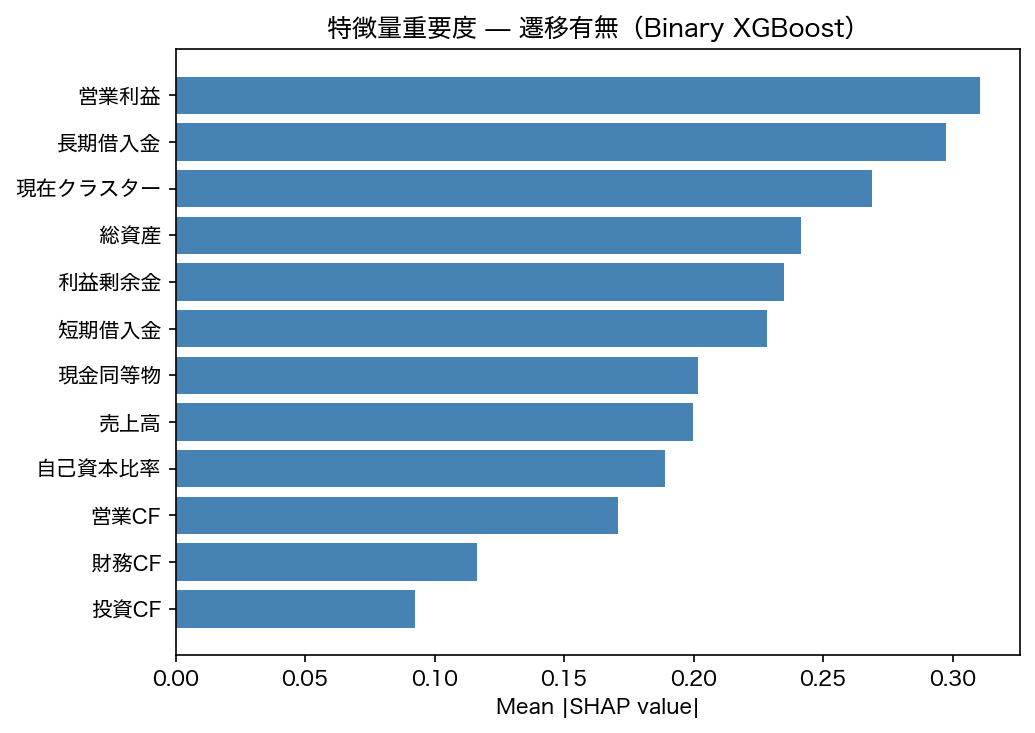
\includegraphics[width=0.70\linewidth]{shap_binary_importance.png}
  \caption{特徴量重要度（Mean $|\mathrm{SHAP}|$）：遷移有無（Binary XGBoost）}
  \label{fig:shap-binary-importance}
\end{figure}

最も重要な特徴量は営業利益（Mean $|\mathrm{SHAP}|$ = 0.311）であり，
次いで長期借入金（0.297），現在クラスター（0.269）が続く。

\subsection{遷移先の多クラス分類（Step 2）}

遷移した企業のみを対象とする多クラス分類の結果を表\ref{tab:mc-performance}に示す。

\begin{table}[htbp]
  \centering
  \caption{Multi-class 分類モデルの性能（Test: 2022〜2024 年度，遷移企業のみ）}
  \label{tab:mc-performance}
  \begin{tabular}{lrrl}
    \toprule
    モデル & Accuracy & AUC-ROC（macro） & 備考 \\
    \midrule
    XGBoost & 0.73 & \textbf{0.947} & 遷移企業のみ（$n=2,081$）\\
    \bottomrule
  \end{tabular}
\end{table}

多クラス分類において AUC（macro） = 0.947 という高い予測精度が達成された。

\subsection{SHAP 分析: 遷移先決定要因}

図\ref{fig:shap-mc-heatmap}に，各遷移先クラスターへの SHAP 値のヒートマップを示す。

\begin{figure}[htbp]
  \centering
  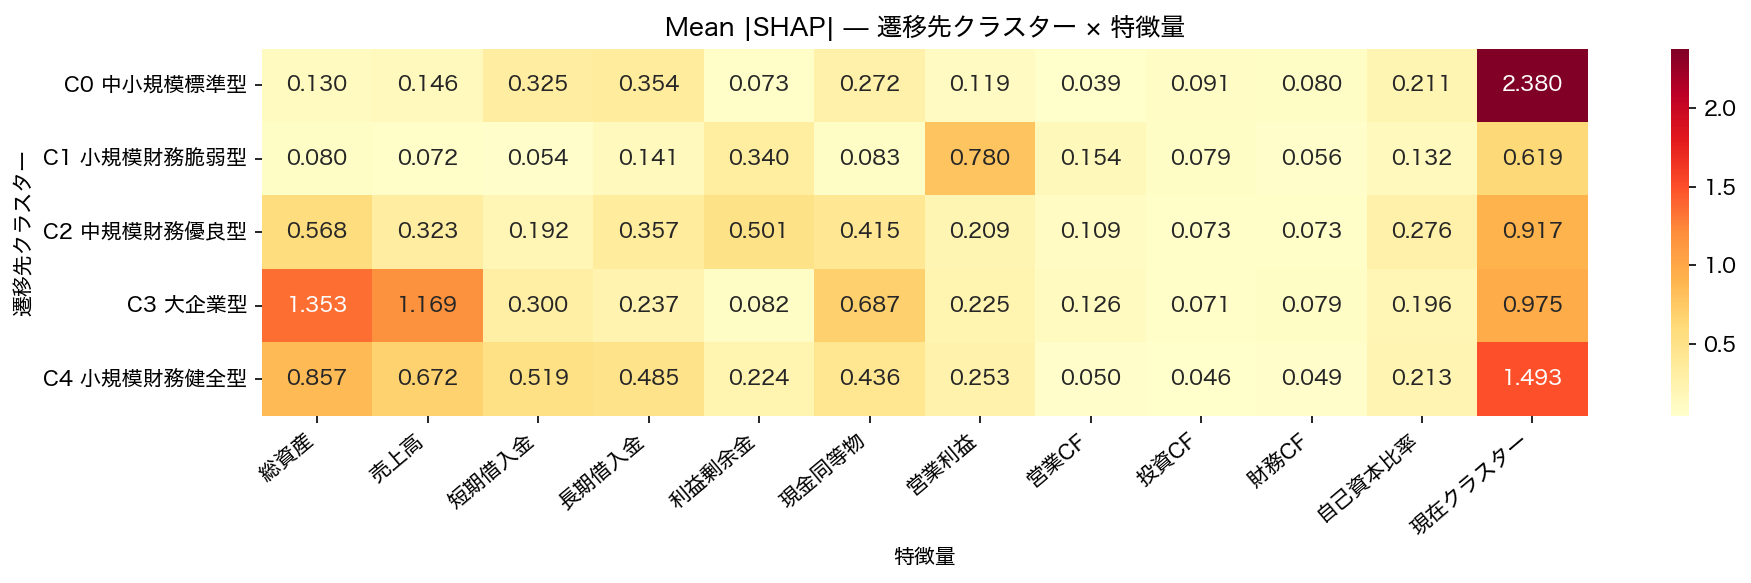
\includegraphics[width=\linewidth]{shap_multiclass_heatmap.png}
  \caption{Mean $|\mathrm{SHAP}|$ ヒートマップ：遷移先クラスター × 特徴量}
  \label{fig:shap-mc-heatmap}
\end{figure}

\section{ロバストネスチェックの結果}
\label{sec:results-robustness}

本節では，PCA の推定期間（全期間 vs 訓練期間のみ）と現在クラスター変数の有無を
組み合わせた 4 パターンの比較分析，および統計的有意性の検定結果を報告する。

\subsection{4 パターン比較}

表\ref{tab:robustness-4pattern}に，PCA 推定期間とクラスター変数の有無を
組み合わせた 4 パターンの予測性能を示す。
図\ref{fig:robustness-4pattern}にその比較を可視化する。

\begin{table}[htbp]
  \centering
  \caption{ロバストネスチェック: 4 パターンの予測性能比較（AUC-ROC）}
  \label{tab:robustness-4pattern}
  \begin{tabular}{llrr}
    \toprule
    パターン & 設定 & Binary & Multi-class \\
    \midrule
    A（基準）& 全期間 PCA + クラスター変数あり & \textbf{0.757} & \textbf{0.947} \\
    B        & Train-only PCA + クラスター変数あり & 0.752 & 0.929 \\
    C        & 全期間 PCA + クラスター変数なし & 0.745 & 0.879 \\
    D        & Train-only PCA + クラスター変数なし & 0.745 & 0.879 \\
    \bottomrule
  \end{tabular}
  \begin{tablenotes}
    \small
    \item 注: Pattern A と B のクラスターラベルは，ハンガリアン法による最適リラベリング後の一致率が 98.4\% であり，実質的に同一のクラスター構造を捉えている。
  \end{tablenotes}
\end{table}

\begin{figure}[htbp]
  \centering
  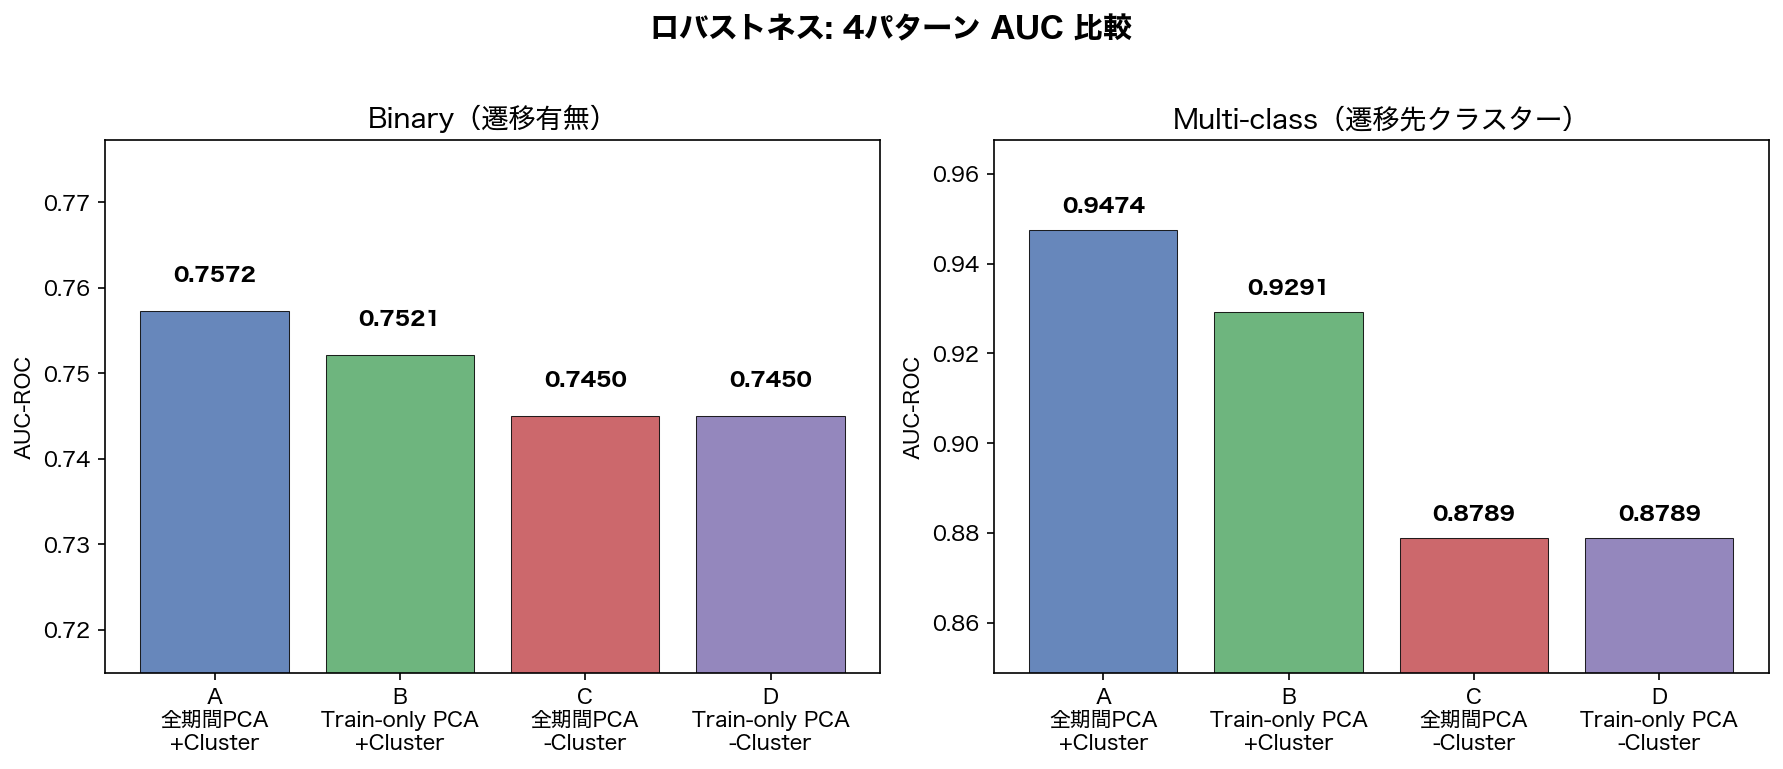
\includegraphics[width=0.85\linewidth]{robustness_4pattern_comparison.png}
  \caption{4 パターンの AUC-ROC 比較（Binary・Multi-class）}
  \label{fig:robustness-4pattern}
\end{figure}

4 パターンの結果から，以下の知見が得られた。
第一に，PCA 推定期間の影響（A vs B）は Binary で 0.005，Multi-class で 0.018 と小さく，
情報漏洩の影響は限定的である。
第二に，現在クラスター変数を除外した場合（A vs C），Binary では 0.012 の低下にとどまり，
財務変数のみでも遷移の有無を相当程度予測できる。
一方，Multi-class では 0.068 の低下が見られ，現在クラスターが遷移先の決定に
重要な役割を果たすこと，すなわちパス依存性の存在を示唆する。
第三に，クラスター変数を除外した場合（C vs D），PCA 推定期間の差異は消失し，
情報漏洩の懸念が現在クラスター変数に限定されることが確認された。

\subsection{統計的有意性の検定}

表\ref{tab:robustness-stat}に，各パターン間の AUC 差に対する
DeLong 検定（Binary）および Bootstrap 95\% 信頼区間（2,000 回リサンプリング）の結果を示す。
図\ref{fig:robustness-stat}に検定結果を可視化する。

\begin{table}[htbp]
  \centering
  \caption{パターン間の AUC 差に対する統計的検定結果}
  \label{tab:robustness-stat}
  \small
  \begin{tabular}{llrrll}
    \toprule
    比較 & 検証内容 & $\Delta$AUC & $p$値 & Bootstrap 95\% CI & 判定 \\
    \midrule
    \multicolumn{6}{l}{\textit{Binary}} \\
    A vs B & PCA 推定期間 & $+0.005$ & 0.121 & $[+0.002, +0.008]$ & n.s. \\
    A vs C & クラスター変数（全期間）& $+0.012$ & 0.040 & $[+0.007, +0.017]$ & $*$ \\
    B vs D & クラスター変数（Train-only）& $+0.007$ & 0.198 & $[+0.003, +0.012]$ & n.s. \\
    C vs D & PCA 推定期間（クラスターなし）& $+0.000$ & 1.000 & $[+0.000, +0.000]$ & n.s. \\
    \midrule
    \multicolumn{6}{l}{\textit{Multi-class（Bootstrap のみ）}} \\
    A vs B & PCA 推定期間 & $+0.018$ & — & $[+0.015, +0.022]$ & $*$ \\
    A vs C & クラスター変数（全期間）& $+0.069$ & — & $[+0.063, +0.074]$ & $*$ \\
    B vs D & クラスター変数（Train-only）& $+0.050$ & — & $[+0.045, +0.056]$ & $*$ \\
    C vs D & PCA 推定期間（クラスターなし）& $+0.000$ & — & $[+0.000, +0.000]$ & n.s. \\
    \bottomrule
  \end{tabular}
  \begin{tablenotes}
    \small
    \item 注: $*$: 95\% 信頼区間が 0 を含まない。n.s.: 非有意。
    DeLong 検定は Binary のみ適用。Multi-class は Bootstrap CI で判定。
  \end{tablenotes}
\end{table}

\begin{figure}[htbp]
  \centering
  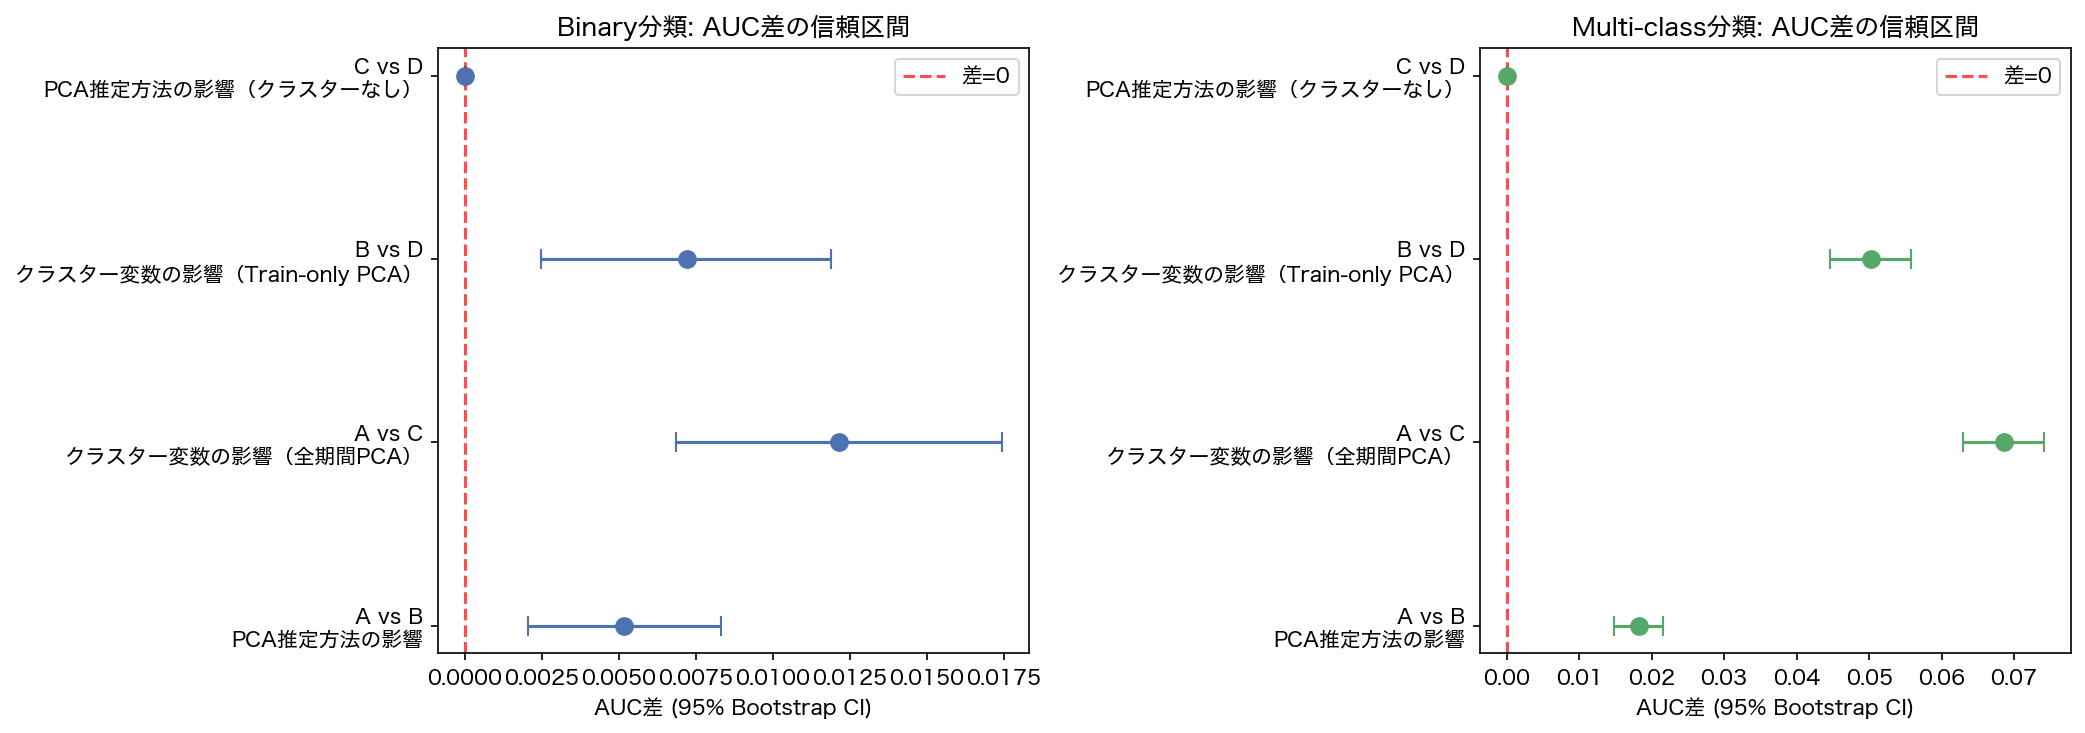
\includegraphics[width=0.85\linewidth]{robustness_stat_test.png}
  \caption{パターン間 AUC 差の統計的検定結果（DeLong $p$値・Bootstrap 95\% CI）}
  \label{fig:robustness-stat}
\end{figure}

DeLong 検定の結果，Binary における PCA 推定期間の影響（A vs B）は統計的に非有意（$p = 0.121$）であり，
情報漏洩が予測精度に実質的な影響を与えていないことが確認された。
クラスター変数の寄与（A vs C）は $p = 0.040$ で有意であるが，
Train-only PCA における同比較（B vs D）では非有意（$p = 0.198$）となり，
クラスター変数の寄与は PCA 推定期間に依存する可能性が示唆された。
Multi-class においては，Bootstrap CI に基づき PCA 推定期間の影響は有意であるものの，
絶対差は 0.018 にとどまり，予測モデルの頑健性が確認された。

%=============================================================
%  第5章 考察
%=============================================================
\chapter{考察}
\label{chap:discussion}

\section{クラスターの経済的解釈}
\label{sec:disc-clusters}

第\ref{sec:results-clusters}節で得られた5クラスターは，
日本上場企業の財務構造の多様性を捉えている。
以下では，各クラスターの経済的背景を考察する。

\paragraph{\Cluster{0}（中小規模・標準型）}
全観測値の 32.5\% を占める最大クラスターであり，
総資産中央値 208 億円，自己資本比率 42.2\% という日本上場企業の標準的な財務プロファイルを示す。
営業利益は正であり，営業キャッシュフローも安定的である。
このクラスターは \tcite{Dickinson2011} の成熟期企業に相当し，
安定した事業基盤を有する中小規模企業の集団と解釈できる。
日本上場企業の約3分の1がこのクラスターに属する事実は，
上場企業の多数が標準的な財務構造を維持していることを示唆する。

\paragraph{\Cluster{1}（小規模・財務脆弱型）}
このクラスターに属する企業は，営業利益が負の値を示す赤字企業を多く含む。
構成比率は 9.9\% と最小であるが，財務的な脆弱性が際立つ。
総資産中央値は 51 億円と小規模であり，収益基盤が不安定な企業群である。
ライフサイクル理論の文脈では，導入期の新興企業や衰退期に入った企業が混在すると
考えられる。\tcite{Habib2017} が示したように，導入期・衰退期の企業は
リスクテイキング水準が高く，財務的な不安定性が構造的に生じやすい。
景気後退期には赤字企業の割合が増加するため，
このクラスターの構成比率はマクロ経済環境に対して敏感に変動する可能性がある。

\paragraph{\Cluster{2}（中規模・財務優良型）}
自己資本比率が 68.7\% と高く，財務の健全性が際立つクラスターである。
総資産中央値は 616 億円と中規模であり，構成比率は 18.0\% を占める。
高い自己資本比率は内部留保の蓄積を反映しており，
\tcite{DeAngelo2006} のライフサイクル仮説における成熟企業の特徴と整合する。
これらの企業は長年の利益蓄積により財務的余裕を確保しており，
外部ショックに対する耐性が高いと考えられる。

\paragraph{\Cluster{3}（大企業型）}
総資産の中央値は約 3,867 億円と突出して大きく，大企業グループを構成する。
構成比率は 21.3\% であり，製造業や金融業の大企業が集積すると考えられる。
自己資本比率は 42.9\% と \Cluster{0} と同水準であるが，
絶対的な資産規模の差異がクラスターの識別に大きく寄与している。
大企業型クラスターの存在は，企業規模がライフサイクル段階とは独立に
財務構造の重要な次元であることを示す。
\tcite{Evans1987} が示した企業規模と成長率の負の関係は，
このクラスターの高い安定性（自己遷移率）と整合する。

\paragraph{\Cluster{4}（小規模・財務健全型）}
規模は小さい（総資産中央値 55 億円）が，自己資本比率 67.2\% と高い財務健全性を持つ。
構成比率は 18.3\% であり，\Cluster{1} と同程度の規模でありながら
対照的な財務体質を示す。
このクラスターは，ニッチ市場で安定した収益を上げる中小企業や，
無借金経営を志向する企業群を含むと考えられる。
\Cluster{1} と \Cluster{4} の対比は，小規模企業の中にも
財務的に健全な企業と脆弱な企業が明確に分かれることを示しており，
企業規模のみでは財務構造を十分に捉えきれないことを裏付ける。

\section{パス依存性と財務慣性}
\label{sec:disc-path-dependence}

本研究で最も顕著な発見の一つは，財務クラスターの強いパス依存性である。
年度間の自己遷移率は平均 80.1\% に達し，企業が同一クラスターに留まる傾向が
極めて強いことが示された。

多項ロジット分析における McFadden の Pseudo $R^2 = 0.637$ は，
遷移先クラスターの説明力の大部分が「現在どのクラスターにいるか」によって
決定されることを示している。
同様に，XGBoost のロバストネスチェック（方法③）において，
クラスター変数を除外すると多クラス分類の AUC が 0.068 低下することも，
この経路依存性を支持する。

この結果は，\tcite{GonzalezRuiz2021} が Markov 連鎖で示した
信用クラスターの持続性と整合し，また \tcite{Pinches1973} が見出した
財務パターンの時系列的安定性を大規模日本企業データで再確認するものである。

このパス依存性を生む潜在的なメカニズムとして，以下の3点が考えられる。

第一に，負債の粘着性（debt overhang）である。
\tcite{Myers1984} が指摘するように，過大な負債を抱える企業は
新規投資のインセンティブが低下し，財務構造の改善が困難になる。
\Cluster{1}（財務脆弱型）の高い自己遷移率は，
この負債の罠（debt trap）メカニズムを反映している可能性がある。

第二に，組織慣性（organizational inertia）の影響がある。
企業の財務戦略は経営者の意思決定パターン，組織文化，
ステークホルダーとの関係に埋め込まれており，
短期的な変更が困難であることが知られている。
\tcite{Hirsch2011} が論じたように，ライフサイクル段階に応じた
負債の最適水準は理論的に異なるが，実際の調整は緩やかにしか進まない。
\tcite{Castro2016} の欧州企業を対象とした研究でも，
目標レバレッジへの調整速度がライフサイクル段階によって異なり，
特に成熟期企業の調整が遅いことが示されている。

第三に，産業構造による固定性がある。
同一産業に属する企業は類似の資産構成・資金需要を有するため，
業種ごとに特定のクラスターへの集積が生じる。
\tcite{Gupta1972} が示したように，産業特性は財務比率のクラスター構造に
強く反映されるため，産業を超えた財務構造の変化は限定的となる。

\section{遷移の非対称性}
\label{sec:disc-asymmetry}

SHAP 分析は，遷移先クラスターによって決定要因が異なるという
重要な非対称性を明らかにした。
この非対称性は，企業の財務構造変化が単一のメカニズムでは説明できないことを示す。

\paragraph{\Cluster{1}（財務脆弱型）への遷移}
最重要変数は営業利益（Mean $|\mathrm{SHAP}|$ が最大）であり，
収益性の悪化（損失転落）が財務脆弱クラスターへの
遷移を促進することが示された。
これは直観的にも理解しやすい：営業赤字は内部留保を毀損し，
資金繰りを悪化させ，財務の脆弱化に直結する。
\tcite{Shumway2001} が倒産予測において収益性指標の重要性を示したことと
整合的であり，収益性の悪化が財務困難の主要なトリガーであることを裏付ける。

\paragraph{\Cluster{0}（標準型）への遷移}
\Cluster{0} への遷移は，多くの場合 \Cluster{2}（財務優良型）や
\Cluster{4}（小規模健全型）からの「下方遷移」として生じる。
自己資本比率の低下や借入金の増加が，優良クラスターから標準クラスターへの
移行を促す要因となる。これは設備投資や事業拡大に伴う
一時的な財務構造の変化を反映している可能性がある。

\paragraph{\Cluster{2}（財務優良型）への遷移}
自己資本比率と利益剰余金が重要な決定要因となる。
内部留保の蓄積により財務体質が改善した企業が，
標準クラスターから財務優良クラスターへと移行する経路を示す。
\tcite{DeAngelo2006} のライフサイクル仮説と整合し，
利益蓄積による企業の成熟化プロセスを捉えている。

\paragraph{\Cluster{3}（大企業型）への遷移}
最重要変数は総資産であり，規模の拡大（M\&A，設備投資）が
大企業クラスターへの遷移を規定することが示された。
\tcite{Owen2010} が示したように，M\&A 活動は企業のライフサイクル段階と
密接に関連しており，成長期から成熟期への移行に伴う規模拡大が
このクラスター遷移の主要な駆動力と考えられる。
営業利益や借入金の SHAP 値は相対的に小さく，
収益性や財務体質よりも規模そのものが遷移を決定する点が特徴的である。

\paragraph{\Cluster{4}（小規模健全型）への遷移}
自己資本比率の上昇と借入金の減少が遷移の主要因となる。
\Cluster{1}（財務脆弱型）からの「回復遷移」として解釈できるケースも含まれ，
財務改善に成功した小規模企業の経路を示す。

以上の非対称性は，財務クラスター遷移の予測において
画一的なモデルではなく，遷移先ごとに異なるメカニズムを
考慮する必要があることを示唆する。
本研究の2段階 XGBoost モデル（遷移有無の二値分類 + 遷移先の多クラス分類）は，
この非対称性に対応した予測フレームワークとして有効に機能している。

\section{含意}
\label{sec:disc-implications}

\subsection{投資家への含意}

本研究の結果は，ポートフォリオ管理と投資判断に対していくつかの含意を持つ。

第一に，財務クラスターの遷移予測は，投資先企業の財務構造変化を事前に察知する
ツールとして活用しうる。AUC = 0.947 の多クラス分類精度は，
遷移先の予測が実用的な水準にあることを示す。
特に，\Cluster{1}（財務脆弱型）への遷移リスクの早期検知は，
ポートフォリオのリスク管理において有用である。

第二に，SHAP 分析で特定された遷移要因（営業利益，長期借入金）は，
投資先企業のモニタリングにおいて重点的に注視すべき指標を示している。
営業利益の急激な悪化は，\Cluster{1} への遷移の先行指標となりうるため，
四半期決算ごとの営業利益の推移は特に注意が必要である。

第三に，80.1\% という高い自己遷移率は，財務クラスターの帰属が
中長期的な投資判断の基盤として利用できることを意味する。
クラスター帰属に基づくポートフォリオ構築は，
従来の産業分類に基づく分散投資を補完する手法となりうる。

\subsection{経営者への含意}

経営者にとって，本研究の最も重要な含意は，
どの財務指標の改善がクラスター遷移（財務体質の改善または悪化）に
最も大きな影響を与えるかを定量的に示した点にある。

SHAP 分析の結果は，営業利益と長期借入金が
クラスター遷移の二大決定要因であることを示している。
したがって，\Cluster{1}（財務脆弱型）からの脱出を目指す経営者は，
まず本業の収益性改善に注力し，次いで長期借入金の適正化を
図ることが合理的な戦略となる。

また，パス依存性の存在は，財務構造の改善が一朝一夕には実現しないことを意味する。
経営者は短期的な財務指標の変動に一喜一憂するのではなく，
中長期的な視点で段階的な財務体質の改善を計画する必要がある。
\tcite{Castro2016} が示した目標レバレッジへの調整速度の遅さは，
この計画的アプローチの重要性を裏付ける。

\subsection{政策立案者への含意}

本研究の結果は，中小企業支援政策に対しても示唆を与える。

第一に，\Cluster{1}（小規模・財務脆弱型）に属する企業は全体の 9.9\% を占め，
これらの企業は赤字基調であり財務的に最も脆弱な集団である。
政策的支援が最も必要とされる対象として，このクラスターに属する企業群を
特定することが可能である。

第二に，遷移要因の分析は，支援施策の設計に有益な情報を提供する。
営業利益の改善が \Cluster{1} からの脱出に最も重要であるとの結果は，
資金繰り支援（融資・補助金）だけでなく，
本業の収益力強化を支援する施策（経営コンサルティング，販路開拓支援等）の
重要性を示唆する。

第三に，パス依存性の存在は，早期介入の重要性を意味する。
企業が財務脆弱クラスターに入った後は，
そこから脱出することが構造的に困難であるため，
財務状況が悪化する前段階での予防的支援が効果的と考えられる。
本研究の遷移予測モデルは，そうした早期警戒システムの基盤として
活用しうる可能性を持つ。

%=============================================================
%  第6章 結論
%=============================================================
\chapter{結論}
\label{chap:conclusion}

\section{研究成果の要約}
\label{sec:conclusion-summary}

本研究では，日本上場企業 \num{3558} 社・15 年間の財務データを用いて，
財務クラスタリングと年度間遷移の分析を行った。主要な成果を以下に要約する。

\begin{enumerate}
  \item \textbf{クラスタリング}:
    PCA と K-Means，およびハンガリアン法の組み合わせにより，
    日本上場企業を5つの財務クラスターに分類した
    （C0:中小規模標準型，C1:小規模財務脆弱型，C2:中規模財務優良型，
    C3:大企業型，C4:小規模財務健全型）。

  \item \textbf{遷移の実態}:
    年度間の自己遷移率は平均 80.1\% であり，企業の財務クラスターは
    年度をまたいで高い安定性を持つ。

  \item \textbf{遷移要因}:
    XGBoost + SHAP 分析により，遷移の主要なトリガーは
    営業利益の変化（Mean $|\mathrm{SHAP}|$ = 0.311）と
    長期借入金の変化（0.297）であることが示された。
    財務変数単独でも AUC = 0.745 の予測精度を達成する。

  \item \textbf{遷移先の決定要因}:
    遷移先クラスターの予測において AUC = 0.947 を達成した。
    C1（財務脆弱型）への遷移は営業利益の悪化，
    C3（大企業型）への遷移は総資産の拡大が主因であることが示された。

  \item \textbf{パス依存性}:
    「現在クラスター」変数が予測において重要な役割を果たすことが確認され，
    財務クラスターの移行には強いパス依存性（経路依存性）が存在することが示された。

  \item \textbf{ロバストネス}:
    PCA 推定期間の相違による AUC 差分は最大 0.018 に留まり，
    分析結果の頑健性が確認された。
\end{enumerate}

\section{学術的貢献}
\label{sec:conclusion-contribution}

本研究の学術的貢献は以下のとおりである。

\begin{enumerate}
  \item ハンガリアン法を用いた年度間ラベル整合型クラスタリング手法を提案した。

  \item 日本上場企業全体を対象とする大規模パネルデータを用いて，
    財務クラスター遷移の実態を記述した初めての研究である。

  \item XGBoost + SHAP を財務クラスター遷移分析に適用し，
    遷移の有無と遷移先の双方を予測・説明する統合的なフレームワークを構築した。
\end{enumerate}

\section{限界と課題}
\label{sec:conclusion-limitations}

本研究にはいくつかの限界がある。

\begin{enumerate}
  \item クラスター数 $K=5$ の選択には主観的な判断が含まれる。
    今後，Bayesian Information Criterion や Gap statistic などの
    客観的指標に基づく選択を検討する余地がある。

  \item 本研究は財務データのみを用いており，経営者の意思決定，
    産業環境，マクロ経済条件などの非財務的要因を考慮していない。

  \item \TODO{その他の限界を記述する}
\end{enumerate}

\section{今後の研究方向}
\label{sec:conclusion-future}

\begin{enumerate}
  \item \textbf{非上場企業への拡張}:
    財務データの入手可能性の問題はあるが，
    非上場企業を含めた分析は研究の外部妥当性を高める。

  \item \textbf{産業別分析}:
    産業ごとにクラスター構造が異なる可能性があり，
    産業分類を考慮した分析が有益である。

  \item \textbf{因果推論への拡張}:
    本研究は予測（予測精度）に焦点を当てており，
    因果効果の識別は行っていない。
    差分の差分法（DID）や操作変数法を用いた因果推論への拡張が考えられる。
\end{enumerate}


%=============================================================
% 参考文献
%=============================================================
\cleardoublepage
\printbibliography[heading=bibintoc, title=参考文献]

%=============================================================
% 付録（必要に応じて）
%=============================================================
% \appendix
% \input{chapters/appendix}

\end{document}
